\documentclass[tikz,border=3pt]{standalone}
\usepackage{amsmath,amssymb,lmodern}
\usetikzlibrary{arrows.meta,calc}

\begin{document}
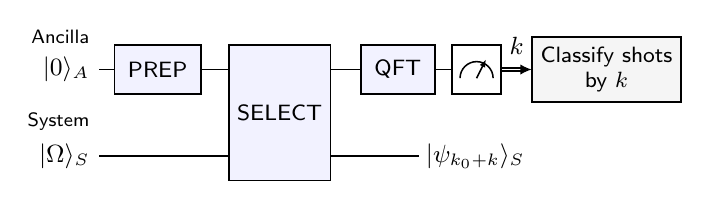
\begin{tikzpicture}[
  x=1cm, y=1cm,
  font=\fontsize{9}{10.5}\selectfont,
  wire/.style={line width=0.55pt},
  gate/.style={
    draw, line width=0.55pt, fill=blue!5,
    minimum height=0.62cm, inner sep=3pt,
    font=\sffamily\fontsize{8}{9}\selectfont
  },
  note/.style={
    align=center, inner sep=0pt,
    font=\sffamily\fontsize{7.5}{9}\selectfont
  },
  classical/.style={
    line width=0.4pt, double=white, double distance=0.7pt,
    -{Latex[length=1.4mm,width=1.3mm]}
  }
]

% Register heights. The ancilla label is encoding-independent.
\def\ya{0.50}
\def\ys{-0.60}

% Inputs.
\node[anchor=east, inner sep=0pt] at (-0.06,\ya)
  {$\lvert 0\rangle_A$};
\node[anchor=east, inner sep=0pt] at (-0.06,\ys)
  {$\lvert\Omega\rangle_S$};
\node[note, anchor=south east] at (-0.06,0.82) {Ancilla};
\node[note, anchor=south east] at (-0.06,-0.28) {System};

% Draw quantum wires first; the filled gates cover their interiors.
\draw[wire] (0.06,\ya) -- (4.85,\ya);
\draw[wire] (0.06,\ys) -- (4.12,\ys);

% Quantum operations. SELECT acts jointly on both registers.
\node[gate, minimum width=1.10cm] (prep) at (0.80,\ya)
  {PREP};
\node[gate, minimum width=1.22cm, minimum height=1.72cm]
  (select) at (2.35,-0.05) {SELECT};
\node[gate, minimum width=0.94cm] (qft) at (3.85,\ya)
  {QFT};

% Functional annotations.
% \node[note, anchor=south] at (0.80,1.03)
%   {Envelope $a_x$\\Phase $k_0$};
% \node[note, anchor=south] at (2.35,1.03)
%   {Controlled\\excitation};
% \node[note, anchor=south] at (3.85,1.03)
%   {Fourier\\transform};

% Ancilla measurement: a meter drawn directly in TikZ.
\node[gate, fill=white, minimum width=0.62cm]
  (measure) at (4.85,\ya) {};
\draw[wire]
  ([xshift=-2.1mm,yshift=-1.1mm]measure.center)
  arc[start angle=180,end angle=0,radius=2.1mm];
\draw[wire,-{Latex[length=1.0mm,width=0.8mm]}]
  ([yshift=-1.1mm]measure.center) --
  ([xshift=1.2mm,yshift=1.3mm]measure.center);

% The measured k is used only in classical post-processing.
\node[gate, fill=black!4, align=center,
      minimum width=1.65cm, minimum height=0.82cm]
  (classify) at (6.50,\ya) {Classify shots\\by $k$};
\draw[classical] (measure.east) --
  node[above=2pt, font=\small] {$k$} (classify.west);


% Conditional system output, not a gate controlled by k.
\node[anchor=west, inner sep=0pt] at (4.20,\ys)
  {$\lvert\psi_{k_0+k}\rangle_S$};

\end{tikzpicture}
\end{document}
